%%%%%%%%%%%%%%%%%%%%%%%%%%%%%%%%%%%%%%%%%%%%%%%%%%%%%%%%%%%%%%%%%%%%%%%%%%%%%%%%%%
\begin{frame}[fragile]\frametitle{}
\begin{center}
{\Large Data Mining}
\end{center}
\end{frame}


%%%%%%%%%%%%%%%%%%%%%%%%%%%%%%%%%%%%%%%%%%%%%%%%%%%%%%%%%%%%%%%%%%%%%%%%%%%%%%%%%%%%
%\begin{frame}[fragile]\frametitle{Data, Data, Everywhere}
%	 \begin{itemize}
%		\item The Famous Five:\\\normalsize
%					  Aural, Visual, Somatic, Gustatory, Olfactory		
%		\item The Social Famous Five:\\\normalsize
%					  What people (like to) hear, see, sense, smell, taste, \ldots
%		\item Manifest Data:\\\normalsize
%					  Likes, Ratings, Reviews, Comments, Views, Searches \ldots
%		\item Data about data:\\\normalsize
%					  Location of a tweet, photo, who called whom, \ldots
%		\item Social data:\\\normalsize
%					  Friend graph, followers, who retweeted, liked,\ldots
%		\item Data about structure:\\\normalsize\vspace{-.4\baselineskip} Layout of the site, In/out links, \ldots 
%	\end{itemize}
%\end{frame}
%	
%%%%%%%%%%%%%%%%%%%%%%%%%%%%%%%%%%%%%%%%%%%%%%%%%%%%%%%%%%%%%%%%%%%%%%%%%%%%%%%%%%%%
%\begin{frame}[fragile]
%	\frametitle{Collecting Digital Data}
%	 \begin{itemize}
%		 \item Proprietary Data collections\\\normalsize
%		 			 Lexis-Nexis, comScore \ldots
%		 \item APIs	\\\normalsize
%		 			 Facebook, \href{http://developer.nytimes.com/docs}{NY Times}, Twitter, Google, FourSquare, \href{dfr.jstor.org}{Jstor}, Zillow \ldots
%	 	 \item Bulk Downloads \\\normalsize
%		 			 Wikipedia, data.gov, IMDB, Million Song Database,  Google n-grams \ldots
%		 \item Scraping
%		 \item Custom Apps\\\normalsize Build custom apps to observe behavior, get (pay) people to download these apps
%	 \end{itemize}
%\end{frame}

%%%%%%%%%%%%%%%%%%%%%%%%%%%%%%%%%%%%%%%%%%%%%%%%%%%%%%%%%%%%%%%%%%%%%%%%%%%%%%%%%%%
\begin{frame}[fragile]
	\frametitle{Scraping}
	 \begin{itemize}
		 \item To analyze data, we typically need structure.\\\normalsize 
		 			  For instance, same number of rows for each column.
		 \item But found data often with human readable structure.
		 \item Copy and paste, type, to a dataset.
		 \item But error prone, and not scalable. 
		 \item \alert{Idea:} Find the less accessible structure, automate based on it.  
	 \end{itemize}
\end{frame}

%%%%%%%%%%%%%%%%%%%%%%%%%%%%%%%%%%%%%%%%%%%%%%%%%%%%%%%%%%%%%%%%%%%%%%%%%%%%%%%%%%%%
%\begin{frame}[fragile]
%	\frametitle{Collecting Found Digital Data}
%	\begin{itemize}
%	 \item Software
%	 			\begin{itemize}
%	 			\item R - Not the best but will do.
%				\item Python, Ruby, Perl, Java, \ldots
%				\item 30 Digits, 80 Legs, Grepsr \ldots
%				\end{itemize}
%	  \item Some things to keep in mind
%	  			\begin{itemize}
%	 			\item Check if there is an API, or if data are available for download
%	 			\item Play Nice: \\
%	 						- Scraper may be disallowed in `robots.txt' \\ 
%	 						- Build lag between requests. \alert{Make lags random.}\\
%	 						- Scrape during off-peak hours
%	 			\end{itemize}
%	 \end{itemize}
%	 			
%\end{frame}
%
%%%%%%%%%%%%%%%%%%%%%%%%%%%%%%%%%%%%%%%%%%%%%%%%%%%%%%%%%%%%%%%%%%%%%%%%%%%%%%%%%%%%
%\begin{frame}[fragile]
%\frametitle{Paper}
%
%	\begin{itemize}
%	\item  Create digital images of paper
%	\item  Identify colored pixels as characters (OCR) 
%	\item  Software
%		\begin{itemize}
%		 \item Adobe Pro., etc. 
%		 \item Best in class commercial: Abbyy FineReader \\
%		 			  Now has an API 
%	 	 \item Best in class open-source: Tesseract
%		\end{itemize}
%	\item Scrape off recognized characters: pyPdf etc.
%	\item Post-processing
%	\end{itemize}
%
%\end{frame}
%
%%%%%%%%%%%%%%%%%%%%%%%%%%%%%%%%%%%%%%%%%%%%%%%%%%%%%%%%%%%%%%%%%%%%%%%%%%%%%%%%%%%%
%\begin{frame}[fragile]
%\frametitle{Pictures, Audio, and Video}
%	\begin{itemize}
%		\item Audio (or Video with audio) to text: Dragon Dictates, Google transcription 
%		\item Pictures: recognize color, faces 
%		\item Objects in images: \href{clarifai.com}{Clarifai}
%		\item Scrape closed-captions
%	\end{itemize}
%\end{frame}
%
%%%%%%%%%%%%%%%%%%%%%%%%%%%%%%%%%%%%%%%%%%%%%%%%%%%%%%%%%%%%%%%%%%%%%%%%%%%%%%%%%%%%
%\begin{frame}[fragile]
%\frametitle{Get Others to Work}
%	\begin{itemize}
%		\item Human Computing
%		\item Amazon.com's Mechanical Turk
%			\begin{itemize}
%				\item  Create Human Intensive Tasks (HITs)
%				\item  \href{https://www.mturk.com/mturk/findhits?match=false}{Surveys, transcription, translation, \ldots}
%				\item  You assess the work and pay out 
%			\end{itemize}
%		\item Odesk, elance, impact sourcing, run your own ads \ldots
%		\item \href{http://www.google.com/insights/consumersurveys/home}{Google} -- surveys as payment for content
%\end{itemize}
%
%\end{frame}
%
%%%%%%%%%%%%%%%%%%%%%%%%%%%%%%%%%%%%%%%%%%%%%%%%%%%%%%%%%%%%%%%%%%%%%%%%%%%%%%%%%%%%
%\begin{frame}[fragile]
%\frametitle{Scraping one HTML page in Python} 
%
%Shakespeare's Twelfth Night\\
%Using \href{http://www.crummy.com/software/BeautifulSoup/}{Beautiful Soup}
%\small
%	\begin{itemize}
%		\item  \lstinline| from BeautifulSoup import BeautifulSoup|
%		\item  \lstinline| from urllib import urlopen|
%		\item 
%		\item  \lstinline| url  = urlopen(`http://bit.ly/1D7wKcH').read()|
%		\item  \lstinline| soup = BeautifulSoup(url)|
%		\item  \lstinline| text = soup.p.contents|
%		\item  \lstinline| print text|
%	\end{itemize}
%\end{frame}
%
%%%%%%%%%%%%%%%%%%%%%%%%%%%%%%%%%%%%%%%%%%%%%%%%%%%%%%%%%%%%%%%%%%%%%%%%%%%%%%%%%%%%
%\begin{frame}[fragile]
%\frametitle{Getting text from one pdf in Python} 
%
%A Political Ad\\
%Using \href{http://pybrary.net/pyPdf/}{PyPdf}
%\small
%	\begin{itemize}
%		\item  \lstinline| import pyPdf|
%		\item 
%		\item  \lstinline| pdf = pyPdf.PdfFileReader(file('path to pdf', `rb'))|
%		\item  \lstinline| content = pdf.getPage(0).extractText()|
%		\item  \lstinline| print content|
%	\end{itemize}
%\end{frame}

%%%%%%%%%%%%%%%%%%%%%%%%%%%%%%%%%%%%%%%%%%%%%%%%%%%%%%%%%%%%%%%%%%%%%%%%%%%%%%%%%%%%
%\begin{frame}[fragile]
%	\frametitle{Scraping many urls/files to structured data}
%	\begin{itemize}
%		\item Loop, exploiting structure of the urls/file paths\\\normalsize 
%					 e.g. \href{http://search.espncricinfo.com/ci/content/match/search.html?search=odi;all=1;page=1}{ESPN URL}
%		\item Handle errors, if files or urls don't open, what do you do?
%		\item To harvest structured data, exploit structure within text
%		\item Trigger words, html tags, \ldots 
%	\end{itemize}
%\end{frame}

%%%%%%%%%%%%%%%%%%%%%%%%%%%%%%%%%%%%%%%%%%%%%%%%%%%%%%%%%%%%%%%%%%%%%%%%%%%%%%%%%%%%
%\begin{frame}[fragile]
%	\frametitle{Exception(al) Handling}
%	\begin{itemize}
%		\item  \lstinline|try:|
%		\item  \lstinline|     pdf = pyPdf.PdfFileReader(file(pdfFile, 'rb'))|
%		\item  \lstinline|except Exception, e:|
%		\item  \lstinline|     return `Cannot Open: {} with error: {}'.format(pdfFile, str(e))|
%	\end{itemize}
%\end{frame}

%%%%%%%%%%%%%%%%%%%%%%%%%%%%%%%%%%%%%%%%%%%%%%%%%%%%%%%%%%%%%%%%%%%%%%%%%%%%%%%%%%%%
%\begin{frame}[fragile]
%	\frametitle{Inside the page}
%	\begin{itemize}
%		\item Chrome Developer Tools
%		\item Quick Tour of HTML
%			\begin{itemize}
%			\item Tags begin with < and end with >
%			\item Tags usually occur in pairs. Some don't (see img). And can be nested.
%			\item \href{https://developer.mozilla.org/en-US/docs/Web/HTML/Element}{Mozilla HTML elements}
%			\item <p> is for paragraph
%			\item <a> is for a link
%			\item <ol>, <ul> is for ordered, unordered list; <li> is a bullet
%			\item tags can have attributes. <a href='http://somesite'></a>
%			\item DOM, hierarchical, parent, child:
%\begin{lstlisting}
%<html>
%    <body>
%        <p></p> 
%    </body>
%</html>
%\end{lstlisting}
%		\end{itemize}
%	\end{itemize}
%\end{frame}
%
%%%%%%%%%%%%%%%%%%%%%%%%%%%%%%%%%%%%%%%%%%%%%%%%%%%%%%%%%%%%%%%%%%%%%%%%%%%%%%%%%%%%
%\begin{frame}[fragile]
%	\frametitle{Find Things}
%	\begin{itemize}
%		\item Navigate by HTML tags:  \lstinline| soup.title, soup.body, soup.body.contents|
%		\item Search HTML tags: 	   \lstinline| soup.find_all('a'), soup.find(id="nav1")|
%		\item 
%		\item So to get all the urls in a page:
%		\item  \lstinline| for link in soup.find_all('a'):|
%		\item  \lstinline|      print(link.get('href'))	|						
%		\item 
%		\item \href{http://www.crummy.com/software/BeautifulSoup/bs4/doc/}{Beautiful Soup Documentation}
%	\end{itemize}
%\end{frame}
%
%%%%%%%%%%%%%%%%%%%%%%%%%%%%%%%%%%%%%%%%%%%%%%%%%%%%%%%%%%%%%%%%%%%%%%%%%%%%%%%%%%%%
%\begin{frame}[fragile]
%	\frametitle{Data Munging}
%	\Large
%		``Data scientists, according to interviews and expert estimates, spend from \alert{50 percent to 80 percent of their time mired in the mundane labor of collecting and preparing data}, before it can be explored for useful information.''\\\vspace{5em}
%
%		\small \href{http://www.nytimes.com/2014/08/18/technology/for-big-data-scientists-hurdle-to-insights-is-janitor-work.html}{New York Times: For BigData Scientists, `Janitor Work' Is Key Hurdle to Insights}
%
%\end{frame}
%
%%%%%%%%%%%%%%%%%%%%%%%%%%%%%%%%%%%%%%%%%%%%%%%%%%%%%%%%%%%%%%%%%%%%%%%%%%%%%%%%%%%%
%\begin{frame}[fragile]
%	\frametitle{Data Munging}
%	\Large
%	``In our experience, the tasks of \alert{exploratory data mining and data cleaning constitute 80\% of the effort} that determines 80\% of the value of the ultimate data.''\\\vspace{5em}
%
%	\small Dasu and Johnson, Exploratory Data Mining and Data Cleaning
%\end{frame}
%
%%%%%%%%%%%%%%%%%%%%%%%%%%%%%%%%%%%%%%%%%%%%%%%%%%%%%%%%%%%%%%%%%%%%%%%%%%%%%%%%%%%%
%\begin{frame}[fragile]
%	\frametitle{Regular (or Rational) Expressions}
%	\begin{itemize}
%		\item  Formal language for specifying text strings
%		\item  Stephen Kleene, `inventor' of regular expressions.
%		\item  Henry Spencer, behind the {\tt regex} library.
%		\item  Descend from {\it finite automata} theory.
%		\item  Matching
%	\end{itemize}
%\end{frame}
%
%%%%%%%%%%%%%%%%%%%%%%%%%%%%%%%%%%%%%%%%%%%%%%%%%%%%%%%%%%%%%%%%%%%%%%%%%%%%%%%%%%%%
%\begin{frame}[fragile]
%	\frametitle{The most basic regular expression}
%	\begin{itemize}
%		\item String literal
%		\item \href{http://regexpal.com}{RegexPal.com}
%		\item Say you are searching for the word apple -- can be uppercase first character, plural, lowercase first character
%	\end{itemize}
%\end{frame}
%
%%%%%%%%%%%%%%%%%%%%%%%%%%%%%%%%%%%%%%%%%%%%%%%%%%%%%%%%%%%%%%%%%%%%%%%%%%%%%%%%%%%%
%\begin{frame}[fragile]
%	\frametitle{Disjunction}
%	\begin{itemize}
%		\item Disjunction, Character classes
%				\begin{itemize}
%				\item   \lstinline| []|
%				\item   \lstinline| [aA]pple matches apple and Apple|
%				\item   \lstinline| [0123456789]  matches any digit|
%				\end{itemize}
%		\item Ranges
%			\begin{itemize}
%				\item   \lstinline| [0-9]  matches any digit|
%				\item   \lstinline| [a-z], [[:lower:]]  matches any lowercase|
%				\item   \lstinline| [a-zA-Z], [[:alpha:]]  matches any uppercase|
%				\item   \lstinline| [a-e1-9]  matches any letter or digit|
%				\item  Hyphen only has a special meaning if used within range.  \lstinline| [-123]|
%			\end{itemize}
%	\end{itemize}
%\end{frame}
%
%%%%%%%%%%%%%%%%%%%%%%%%%%%%%%%%%%%%%%%%%%%%%%%%%%%%%%%%%%%%%%%%%%%%%%%%%%%%%%%%%%%%
%\begin{frame}[fragile]
%	\frametitle{Disjunction Contd..}
%	\begin{itemize}
%	\item Negation in Disjunction\\\normalsize
%			\begin{itemize}
%			\item   \lstinline| ^ right after the square bracket means a negation|
%			\item   \lstinline|  [^A-Z]|
%			\item   \lstinline|  [^Aa] means neither a capital A nor a lowercase a|
%			\item   \lstinline|  [^e^] means not an e, and not ^|
%			\end{itemize}
%	\item Disjunction for longer strings\\\normalsize
%			\begin{itemize}
%			    \item   \lstinline|  pipe|
%				\item   \lstinline|  a|b|c = [abc]|
%				\item   \lstinline|  apple|pie|
%				\item   \lstinline|  [aA]pple|[aA]nd|
%			\end{itemize}
%	\end{itemize}
%\end{frame}
%
%%%%%%%%%%%%%%%%%%%%%%%%%%%%%%%%%%%%%%%%%%%%%%%%%%%%%%%%%%%%%%%%%%%%%%%%%%%%%%%%%%%%
%\begin{frame}[fragile]
%	\frametitle{Special characters}
%	\begin{itemize}
%	\item ? - previous character is optional: colou?r - color, colour
%	\item  . matches any character\\
%				  e.g. beg.n matches begun, begin, began
%	\item Kleene Operators - named after Steven Kleene
%			\begin{itemize}
%			\item *  matches 0 or more of the previous characters\\
%						e.g. oo*h will match ooh, oooh, etc.\\
%						(abc)* will match abc, abcabc, etc.
%			\item +  matches 1 or more of the previous characters\\
%						e.g. o+h will match ooh, oooh, etc. 
%			\end{itemize}
%	\end{itemize}
%\end{frame}
%
%%%%%%%%%%%%%%%%%%%%%%%%%%%%%%%%%%%%%%%%%%%%%%%%%%%%%%%%%%%%%%%%%%%%%%%%%%%%%%%%%%%%
%\begin{frame}[fragile]
%	\frametitle{Repetition Ranges}
%	\begin{itemize}
%	\item  Specific ranges can also be specified
%	\item  \small  \lstinline| { } to specify range for the immediately preceding regex|
%	\item   \lstinline| {n}  means exactly n occurrences|
%	\item   \lstinline| {n,} means at least n occurrences|
%	\item   \lstinline| {n,m} means at least n and no more than m occurrences|
%	\item  Example:  \lstinline| . {0, } = .*|	
%	\end{itemize}
%\end{frame}
%
%%%%%%%%%%%%%%%%%%%%%%%%%%%%%%%%%%%%%%%%%%%%%%%%%%%%%%%%%%%%%%%%%%%%%%%%%%%%%%%%%%%%
%\begin{frame}[fragile]\frametitle{More Regex}
%		\begin{itemize}
%	\item Anchors
%			\begin{itemize}
%			\item  \^ matches the beginning of the line \\
%	 			  e.g.  \lstinline| ^[A-Z] matches a capital letter at the start of a line.|
%			\item  \$ matches the end of the line.
%			\end{itemize}
%	\item   \lstinline| \. means a period| 
%	\item  Example: look for the word `the'
%	\begin{itemize}
%		\item missed capitalization: [tT]he
%		\item make pattern more precise: \\
%					 \lstinline| [tT]he[^A-Za-z], ^[tT]he[^A-Za-z]|
%	\end{itemize}
%	\end{itemize}
%\end{frame}
%
%%%%%%%%%%%%%%%%%%%%%%%%%%%%%%%%%%%%%%%%%%%%%%%%%%%%%%%%%%%%%%%%%%%%%%%%%%%%%%%%%%%%
%\begin{frame}[fragile]
%\frametitle{False Positive and Negatives}
%	\begin{itemize}
%	\item False positives or Type 1 errors - matching things we shouldn't match
%	\item False negatives or Type 2 errors - not matching things we should match
%	\item Cost attached to false negative and positive
%	\item Provide some metrics by comparing against good data for a small sample
%	\end{itemize}
%\end{frame}
%
%%%%%%%%%%%%%%%%%%%%%%%%%%%%%%%%%%%%%%%%%%%%%%%%%%%%%%%%%%%%%%%%%%%%%%%%%%%%%%%%%%%%
%\begin{frame}[fragile]
%	\frametitle{Edit Distance}
%	\begin{itemize}
%		\item pwned -> owned or pawned?
%		\item standd -> strand, stand, stood, or sand?
%		\item How similar are two strings?
%		\item Applications
%			\begin{itemize}
%			\item Spell Correction
%			\item Also comes up in computational biology
%			\item Machine translation
%			\item Information extraction
%			\item Speech recognition
%			\end{itemize}
%	\end{itemize}
%\end{frame}
%
%%%%%%%%%%%%%%%%%%%%%%%%%%%%%%%%%%%%%%%%%%%%%%%%%%%%%%%%%%%%%%%%%%%%%%%%%%%%%%%%%%%%
%\begin{frame}[fragile]
%	\frametitle{Edit Distance}
%	\begin{itemize}
%		\item Typically refers to minimum edit distance
%		\item Minimum number of editing operations to convert one string to another
%			\begin{itemize}
%				\item Insertion
%				\item Deletion
%				\item Substitution
%			\end{itemize}
%		\item e.g. two strings: intention, execution 
%			\begin{itemize}
%				\item align it with second letter
%				\item d (delete), s (substitute), s, i(nsert), s
%				\item if each operation costs 1, edit distance = 5
%				\item if substitition cost 2 (levenshtein distance), distance = 8
%			\end{itemize}
%		\item You can implement this at word level so Microsoft Corp. is 1 away from Microsoft.
%	\end{itemize}
%\end{frame}
%
%%%%%%%%%%%%%%%%%%%%%%%%%%%%%%%%%%%%%%%%%%%%%%%%%%%%%%%%%%%%%%%%%%%%%%%%%%%%%%%%%%%%
%\begin{frame}[fragile]
%	\frametitle{Text as Data}
%	\begin{itemize}
%		\item Bag of words assumption\\\normalsize
%					Lose word order
%		\item Remove stop words:\\\normalsize
%					If, and, but, who, what, the, they, their, a, or, \ldots\\
%					\alert{Be careful: one person's stopword is another's key term.}
%		\item (Same) Word: Stemming and Lemmatization\\\normalsize
%					Taxing, taxes, taxation, taxable $\leadsto$ tax
%		\item Remove rare words\\\normalsize
%					$\sim$ .5\% to 15\%, depending on application\\
%		\item Convert to lowercase, drop numbers, punctuation, etc.
%	\end{itemize}
%\end{frame}
%
%%%%%%%%%%%%%%%%%%%%%%%%%%%%%%%%%%%%%%%%%%%%%%%%%%%%%%%%%%%%%%%%%%%%%%%%%%%%%%%%%%%%
%\begin{frame}[fragile]
%	\frametitle{How?}
%	Using Natural Language Toolkit (\tt{nltk})
%	\begin{itemize}
%			\item \textbf{Lowercase}: 
% 					 	 \lstinline|text = text.lower()| 
% 			\item \textbf{Remove stop words}:
%	 			\item  \lstinline|swords = stopwords.words('english')|
%	 			\item  \lstinline|words  = wordpunct_tokenize(text)|
%	 			\item  \lstinline|words  = [w for w in words if w not in swords]|
%	    		\item  \lstinline|text = ' '.join(words)|
% 			\item \textbf{Stemming}: 
% 				\item  \lstinline|st = EnglishStemmer()|
% 				\item  \lstinline|words = wordpunct_tokenize(text)|
%    			\item  \lstinline|words = [st.stem(w) for w in words]|
%    			\item  \lstinline|text = ' '.join(words)|
%		\end{itemize}
%\end{frame}
%
%%%%%%%%%%%%%%%%%%%%%%%%%%%%%%%%%%%%%%%%%%%%%%%%%%%%%%%%%%%%%%%%%%%%%%%%%%%%%%%%%%%%
%\begin{frame}[fragile]
%	\frametitle{To Matrices}
%	\begin{itemize}
%			\item n-grams
%					 \lstinline|
%						from nltk import bigrams, trigrams, ngrams
%						text = word tokenize(text)
%						text_bi  = bigrams(text)
%					|
%	\end{itemize}
%\end{frame}

%%%%%%%%%%%%%%%%%%%%%%%%%%%%%%%%%%%%%%%%%%%%%%%%%%%%%%%%%%%%%%%%%%%%%%%%%%%%%%%%%%%
\begin{frame}[fragile]\frametitle{Web Scraping Workflow}
Web scraping downloads and processes content from the Web
\begin{itemize}
\item Get the website - using HTTP library
\item Parse the html document - using any parsing library
\item Store the results - either a db, csv, text file, etc
\end{itemize}
Libraries:
\begin{itemize}
\item \textbf{Requests}: Downloads files and web pages from the Internet
\item \textbf{Beautiful Soup}: Parses HTML, the format that web pages are written in.
\item \textbf{Selenium}: To fill in forms and simulate mouse clicks in this browser.
\end{itemize}
\end{frame}

%%%%%%%%%%%%%%%%%%%%%%%%%%%%%%%%%%%%%%%%%%%%%%%%%%%%%%%%%%%%%%%%%%%%%%%%%%%%%%%%%%%
\begin{frame}[fragile]\frametitle{Web Scraping Issues}
Web-scraping is difficult for some annoying (i.e. not particularly intellectually challenging) reasons:
\begin{itemize}
\item Web pages change frequently and will break your code.
\item Web page source code is often not logical and consistent (major browsers are incredibly good at overlooking this, but python and your own code probably aren't).
\item Content may be different for different User Agents (which client you're using).
\item Content may be hidden behind logins, require cookies or other fancier browser options, etc.
\item Websites may attempt to limit automated crawling of their pages (robots.txt) — your code may have to go out of its way to be nice, or risk getting banned.
\end{itemize}
\end{frame}

%%%%%%%%%%%%%%%%%%%%%%%%%%%%%%%%%%%%%%%%%%%%%%%%%%%%%%%%%%%%%%%%%%%%%%%%%%%%%%%%%%%
\begin{frame}[fragile]\frametitle{Web Scraping: Get the website }
Suppose that we want to crawl this web page:
https://www.hkex.com.hk/eng/index.htm

\begin{center}
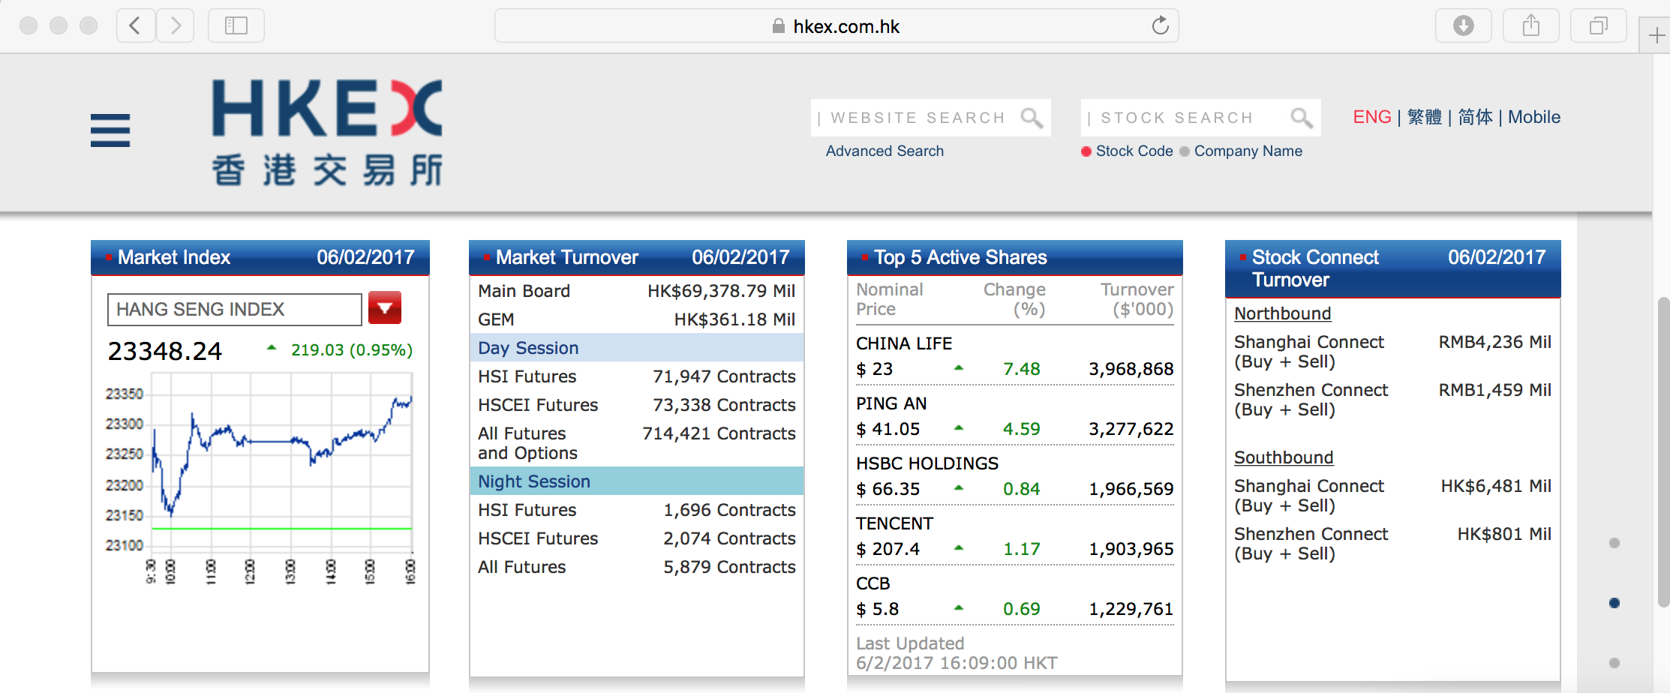
\includegraphics[width=\linewidth,keepaspectratio]{hkex}
\end{center}
\tiny{(Reference: https://studyslide.com/doc/288619/tutorial-2---hkust-cse)}

\end{frame}

%%%%%%%%%%%%%%%%%%%%%%%%%%%%%%%%%%%%%%%%%%%%%%%%%%%%%%%%%%%%%%%%%%%%%%%%%%%%%%%%%%%
\begin{frame}[fragile]\frametitle{Web Scraping: Get the website }
In Chrome: Right-click, choose ``View Page Source''
\begin{center}
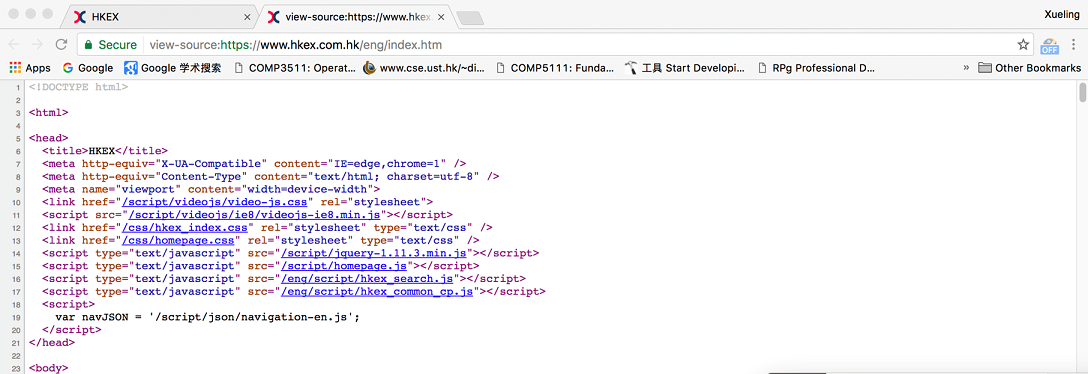
\includegraphics[width=\linewidth,keepaspectratio]{hkexsrc}
\end{center}
\end{frame}

%%%%%%%%%%%%%%%%%%%%%%%%%%%%%%%%%%%%%%%%%%%%%%%%%%%%%%%%%%%%%%%%%%%%%%%%%%%%%%%%%%%
\begin{frame}[fragile]\frametitle{Web Scraping: Get the website }
We need to collect useful information from source HTML code:
\begin{center}
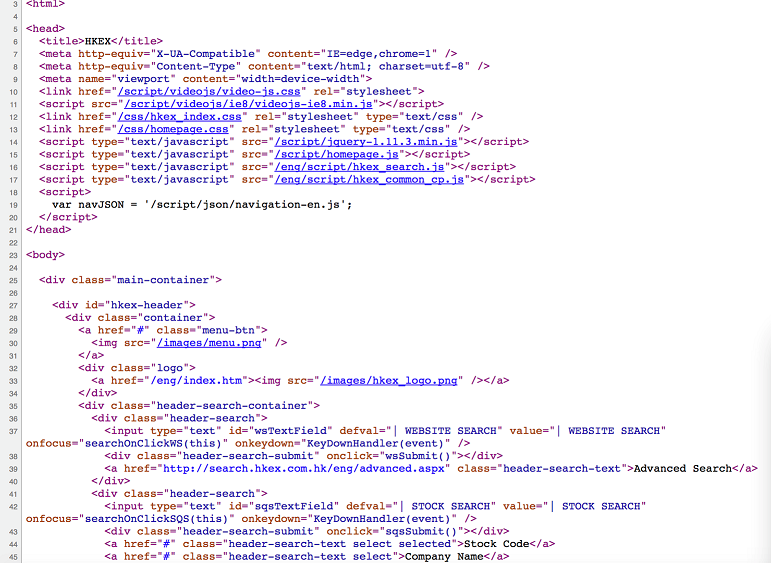
\includegraphics[width=0.8\linewidth,keepaspectratio]{hkexhtml}
\end{center}
\end{frame}


%%%%%%%%%%%%%%%%%%%%%%%%%%%%%%%%%%%%%%%%%%%%%%%%%%%%%%%%%%%%%%%%%%%%%%%%%%%%%%%%%%%
\begin{frame}[fragile]\frametitle{Requests}
Web scraping downloads and processes content from the Web
\begin{itemize}
\item Do not need to worry about complicated issues such as network errors, connection problems, and data compression.
\item \lstinline|requests.get()| function takes a string of a URL to download. 
\begin{lstlisting}
import requests
res = requests.get('https://automatetheboringstuff.com/files/rj.txt')
\end{lstlisting}
\item Response contains the response that the web server gave.
\begin{lstlisting}
if res.status_code == requests.codes.ok:
	print(res.text)
\end{lstlisting}
\end{itemize}
\end{frame}
%%%%%%%%%%%%%%%%%%%%%%%%%%%%%%%%%%%%%%%%%%%%%%%%%%%%%%%%%%%%%%%%%%%%%%%%%%%%%%%%%%%
\begin{frame}[fragile]\frametitle{Beautiful Soup}
Web scraping downloads and processes content from the Web
\begin{itemize}
\item To parse a document, pass it into the BeautifulSoup constructor. You can pass in a string or an open filehandle:

\begin{lstlisting}
from bs4 import BeautifulSoup

soup = BeautifulSoup(open("index.html")) 
soup = BeautifulSoup("<html>data</html>")  
\end{lstlisting}
\item Print the content in the soup object in better format 
\lstinline|print(soup.prettify())|
\item A Tag object corresponds to an XML or HTML tag in the original document:
\lstinline|<title>The Dormouse's story</title>|
\item Use BeautifulSoup to get the tags in a convenient way
\lstinline|print(soup.title)| \\
\lstinline|print(soup.head)|
\end{itemize}

\end{frame}

%%%%%%%%%%%%%%%%%%%%%%%%%%%%%%%%%%%%%%%%%%%%%%%%%%%%%%%%%%%%%%%%%%%%%%%%%%%%%%%%%%%
\begin{frame}[fragile]\frametitle{Beautiful Soup: Tag}
Web scraping downloads and processes content from the Web
\begin{itemize}
\item Every tag has a name, accessible as .name
\begin{lstlisting}
print(soup.head.name)
#head
\end{lstlisting}
\item  A tag may have any number of attributes. The tag \lstinline|<b class=``boldest''>| has an attribute ``class'' whose value is ``boldest''. You can access a tag's attributes by treating the tag like a dictionary:
\begin{lstlisting}
print(soup.p.attrs)
#{'class': ['title'], 'name': 'dromouse'}
print(soup.p['class'])
#['title']
print(soup.p.get('class'))
#['title']
print(type(soup.p))
#<class 'bs4.element.Tag'>
\end{lstlisting}
\end{itemize}

\end{frame}

%%%%%%%%%%%%%%%%%%%%%%%%%%%%%%%%%%%%%%%%%%%%%%%%%%%%%%%%%%%%%%%%%%%%%%%%%%%%%%%%%%%
\begin{frame}[fragile]\frametitle{Beautiful Soup: Sample workflow}

\begin{itemize}
\item To begin, we need to import Beautiful Soup and urllib, and grab source code:
\begin{lstlisting}
import bs4 as bs
import urllib.request

source = urllib.request.urlopen('https://pythonprogramming.net/parsememcparseface/').read()
\end{lstlisting}
\item  Then, we create the ``soup''. This is a beautiful soup object:
\begin{lstlisting}
soup = bs.BeautifulSoup(source,'lxml')
\end{lstlisting}
\item  Find more about whats in the soup object:
\begin{lstlisting}
print(soup.title)
print(soup.title.name)
print(soup.title.string)

# beginning navigation:
print(soup.title.parent.name)

# getting specific values:
print(soup.p)
\end{lstlisting}
\end{itemize}

\end{frame}

%%%%%%%%%%%%%%%%%%%%%%%%%%%%%%%%%%%%%%%%%%%%%%%%%%%%%%%%%%%%%%%%%%%%%%%%%%%%%%%%%%%
\begin{frame}[fragile]\frametitle{Beautiful Soup: Sample workflow}

\begin{itemize}
\item Finding paragraph tags <p> is a fairly common task. What if we wanted to find them all?
\begin{lstlisting}
print(soup.find_all('p'))
\end{lstlisting}
\item  We can also iterate through them:
\begin{lstlisting}
for paragraph in soup.find_all('p'):
    print(paragraph.string)
    print(str(paragraph.text))
\end{lstlisting}
\item  The difference between string and text is that string produces a NavigableString object, and text is just typical unicode text. 
\item  Notice that, if there are child tags in the paragraph item that we're attempting to use .string on, we will get None returned.
\end{itemize}

\end{frame}

%%%%%%%%%%%%%%%%%%%%%%%%%%%%%%%%%%%%%%%%%%%%%%%%%%%%%%%%%%%%%%%%%%%%%%%%%%%%%%%%%%%
\begin{frame}[fragile]\frametitle{Beautiful Soup: Sample workflow}

\begin{itemize}
\item  Another common task is to grab links. For example:
\begin{lstlisting}
for url in soup.find_all('a'):
    print(url.get('href'))
\end{lstlisting}
\item  In this case, if we just grabbed the .text from the tag, you'd get the anchor text, but we actually want the link itself. 
\item  That's why we're using \lstinline|.get('href')| to get the true URL.
\item Finally, you may just want to grab text. You can use \lstinline|.get_text()| on a Beautiful Soup object, including the full soup:
\begin{lstlisting}
print(soup.get_text())
\end{lstlisting}
\end{itemize}
This concludes the introduction to Beautiful Soup. 
\end{frame}

%%%%%%%%%%%%%%%%%%%%%%%%%%%%%%%%%%%%%%%%%%%%%%%%%%%%%%%%%%%%%%%%%%%%%%%%%%%%%%%%%%%
\begin{frame}[fragile]\frametitle{Beautiful Soup: Sample workflow}

\begin{itemize}
\item  Another common task is to grab links. For example:
\begin{lstlisting}
for url in soup.find_all('a'):
    print(url.get('href'))
\end{lstlisting}
\item  In this case, if we just grabbed the .text from the tag, you'd get the anchor text, but we actually want the link itself. 
\item  That's why we're using \lstinline|.get('href')| to get the true URL.
\item Finally, you may just want to grab text. You can use \lstinline|.get_text()| on a Beautiful Soup object, including the full soup:
\begin{lstlisting}
print(soup.get_text())
\end{lstlisting}
\end{itemize}
This concludes the introduction to Beautiful Soup. Next is the Navigation.
\end{frame}


%%%%%%%%%%%%%%%%%%%%%%%%%%%%%%%%%%%%%%%%%%%%%%%%%%%%%%%%%%%%%%%%%%%%%%%%%%%%%%%%%%%
\begin{frame}[fragile]\frametitle{Beautiful Soup: Sample workflow}

\begin{itemize}
\item  In this case, we're grabbing the first nav tags that we can find (the navigation bar):
\begin{lstlisting}
nav = soup.nav
for url in nav.find_all('a'):
    print(url.get('href'))
\end{lstlisting}
\item   You could also go for soup.body to get the body section, then grab the \lstinline|.text| from there:
\begin{lstlisting}
body = soup.body
for paragraph in body.find_all('p'):
    print(paragraph.text)
\end{lstlisting}
\item To avoid multiple tags with same names, use other things such as classes, to differentiate:
\begin{lstlisting}
for div in soup.find_all('div', class_='body'):
    print(div.text)
\end{lstlisting}
\end{itemize}

\end{frame}

%%%%%%%%%%%%%%%%%%%%%%%%%%%%%%%%%%%%%%%%%%%%%%%%%%%%%%%%%%%%%%%%%%%%%%%%%%%%%%%%%%%
\begin{frame}[fragile]\frametitle{Beautiful Soup: Sample workflow}

\begin{itemize}
\item Parsing the table:
\begin{lstlisting}
table = soup.find('table')
\end{lstlisting}
\item   Next, we can find the table rows within the table:
\begin{lstlisting}
table_rows = table.find_all('tr')
\end{lstlisting}
\item Then we can iterate through the rows, find the td tags, and then print out each of the table data tags:
\begin{lstlisting}
for tr in table_rows:
    td = tr.find_all('td')
    row = [i.text for i in td]
    print(row)
\end{lstlisting}
\end{itemize}

\end{frame}







